\section{完成情况及性能参数}
\subsection{整体介绍}
在原图界面伸出食指和中指，系统确认手势后选择第2号风格，HDMI屏自动显示彩色剪纸。回到左右对比界面，移动镜头前的物体，同一帧的轮廓可以横跨中线连续显示。

\subsection{赛题要求与完成情况}
系统在Ti60上完成了从摄像头原始像素到风格画面的处理。SC431HAI输出1920×1080 RAW10，FPGA将其转换为1280×720 RGB565图像。卷积网络在这一分辨率上逐像素生成风格结果，HDMI提供全屏原图、全屏风格和左原右风格三种视图。

\begin{table}[H]\centering\small
\caption{实时绘画赛题的设计要求与系统实现}\label{tab:contest}
\begin{tabularx}{\linewidth}{@{}p{.20\linewidth}p{.31\linewidth}X@{}}\toprule
功能 & 赛题要求 & 系统实现及已有结果\\\midrule
采集与预处理 & MIPI CSI-2，至少640×480、30帧/秒 & 四通道接收RAW10，完成包校验、Bayer插值及720p缩放。每发布一幅好帧更新采集计数。\\
外部帧缓存 & 双缓冲保存完整帧，保障采集连续 & DDR3设置三个原图槽、三个输出槽。采集、推理和显示分别持有所用帧，记录跳帧、坏帧和欠载。\\
卷积加速与控制 & 3×3或5×5卷积、激活和归一化，总线读写DDR，RISC-V调度 & FPGA实现3×3深度卷积、1×1通道混合和饱和激活，BN折叠入卷积。RISC-V配置摄像头、加载参数，管理作业与完成中断。\\
显示与对比 & 720p60或1080p30，原画对比及FPS叠加 & HDMI使用74.25\,MHz像素时钟输出720p60。左右两侧取自同一源帧，屏显C、I分别给出采集和推理帧率。\\
处理速度 & 基础目标为640×480稳定超过15帧/秒，高阶目标为720p达到30帧/秒 & 720p槽0对比模式的CNN/DMA整帧仿真处理921600像素，耗时25.585\,ms，折合39.085帧/秒。\\
多风格与模型规模 & 至少两种风格，切换低于100\,ms且不丢帧，模型小于500\,KB & 十组风格共用一个加速器。每风格567个可训练参数、396个卷积系数，十组部署参数共7360字节。支持按键及手势选画。\\\bottomrule
\end{tabularx}\end{table}
整机持续帧率、丢帧数和按键切换延迟尚待现场实测。

\subsection{工程成果}
\subsubsection{机械与电路成果}
摄像头以排线连接J4，HDMI输出端连接显示器，USB串口连接测量主机。配置审查覆盖79个物理端口及12组Bank，逐项核对信号方向、电压域和DDR数据选通。实物连接与运行画面在本章实拍栏中记录。

\subsubsection{软件成果}
十个风格分支共5670个可训练参数。离线程序将各分支导出为整数参数包，板上10588字节的RISC-V固件负责选择参数、调度推理和处理手势请求。CAM7串口输出帧数、作业周期和交互状态。

\subsection{资源占用与处理性能}
布局布线后，整机使用142个DSP和230块RAM10。DSP承担卷积乘加，RAM10用于行缓存、像素队列、处理器存储和手势快照。图\ref{fig:utilization}给出三类主要资源的占比。逻辑资源XLR的使用率最高，为97.06\%。整机使用29702个寄存器和32898个查找表，I3时序模型下最小建立、保持余量分别为+0.108\,ns和+0.026\,ns。
\begin{figure}[H]\centering
\begin{tikzpicture}[x=1cm,y=.80cm,font=\small]
\foreach \y/\name/\used/\total/\pc in {2/RAM10/230/256/89.84,1/DSP/142/160/88.75,0/XLR/59011/60800/97.06}{
 \node[anchor=east] at (-.17,\y+.23){\name};
 \fill[navy!9] (0,\y) rectangle (7.0,\y+.48);
 \fill[teal!85] (0,\y) rectangle ({.07*\pc},\y+.48);
 \node[anchor=west,font=\footnotesize] at (7.13,\y+.23){\used\,/\,\total\quad(\pc\%)};
}
\node[anchor=west,font=\footnotesize] at (0,-.42){已用资源占器件总量的比例};
\end{tikzpicture}
\caption{Ti60F225I3布局布线后的资源占用。十个风格槽共享同一组卷积算子和行缓存。}\label{fig:utilization}
\end{figure}

梵高风格的完整720p对比帧在CNN/DMA仿真中用时2558528个100\,MHz时钟周期。921600个输出像素与整数参考逐点一致。该时间包含条带运算、读写背压和最后一次写响应，对应每帧25.585\,ms。板上运行时，信息层从采集与推理计数器取数，在消隐期同步到显示端，如图\ref{fig:rates-ui}所示。

\begin{figure}[H]\centering
\begin{tikzpicture}[x=1cm,y=1cm,font=\small,
 stage/.style={draw=navy!65,rounded corners=2pt,fill=pale,align=center,inner sep=4pt},
 arrow/.style={-{Stealth[length=2mm]},draw=teal,thick}]
\node[stage,minimum width=3.65cm] (cap) at (0,1.12) {源帧成功发布};
\node[stage,minimum width=3.65cm] (cnn) at (0,0) {风格帧写回完成};
\node[stage] (dc) at (4.1,1.12) {采集计数每秒增量};
\node[stage] (di) at (4.1,0) {推理计数每秒增量};
\node[stage,fill=teal!12] (c) at (7.95,1.12) {屏显 C};
\node[stage,fill=teal!12] (i) at (7.95,0) {屏显 I};
\draw[arrow] (cap)--(dc);\draw[arrow] (cnn)--(di);\draw[arrow] (dc)--(c);\draw[arrow] (di)--(i);
\node[stage,minimum width=3.65cm] (clock) at (0,-1.18) {像素时钟74.25\,MHz};
\node[stage] (scan) at (4.1,-1.18) {每帧$1650\times750$拍};
\node[stage,fill=orange!13] (h) at (7.95,-1.18) {屏显 H60};
\draw[arrow] (clock)--(scan);\draw[arrow] (scan)--(h);
\end{tikzpicture}
\caption{屏幕三项速率的来源。C与I分别由完整采集和神经作业完成事件得到，H60由视频扫描时序确定。}\label{fig:rates-ui}
\end{figure}

十组参数均通过小尺寸RTL与映射算子逐值核对。RISC-V固件仿真覆盖十槽加载，共完成2160项参数写入。手势全流程验证依次输入3张空背景、40张个人模板和15张识别快照，经过4.08秒的确认窗口后，固件提交对应风格请求。

\clearpage
\subsection{十风格训练效果}
两张公共领域作品《蒙娜丽莎》和《戴珍珠耳环的少女》分别由来源页面获取\cite{mona,pearl}，在十组参数上保持相同输入，便于比较风格差异。每张原作按比例缩至高720像素，两侧反射补边为1280×720后量化RGB565，再运行当前最终整数模型；下图仅裁出原画有效区域，不改变模型输出颜色或锐度。

以下各图从左至右依次为《蒙娜丽莎》原图与转换图、《戴珍珠耳环的少女》原图与转换图。观察同一处发丝、衣褶和背景，可以比较不同参数对轮廓、明暗与短笔触的处理。


\begin{figure}[H]\centering
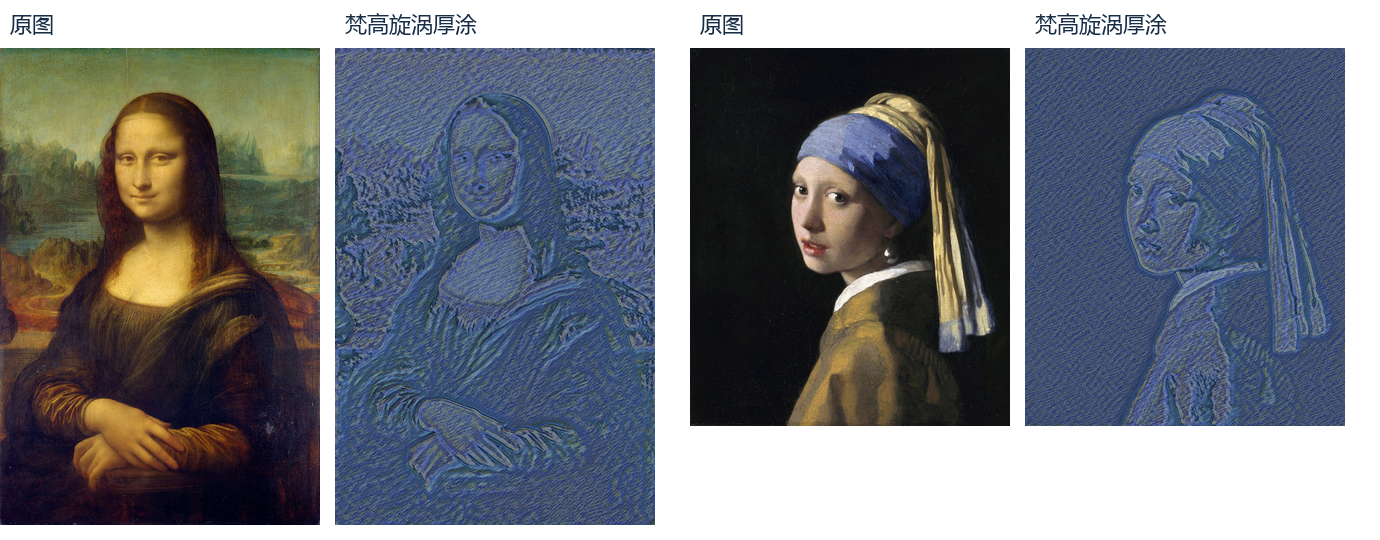
\includegraphics[width=\linewidth]{assets/comparisons/style_00_pairs.png}
\caption{槽0 梵高旋涡厚涂}
\end{figure}
\begin{figure}[H]\centering
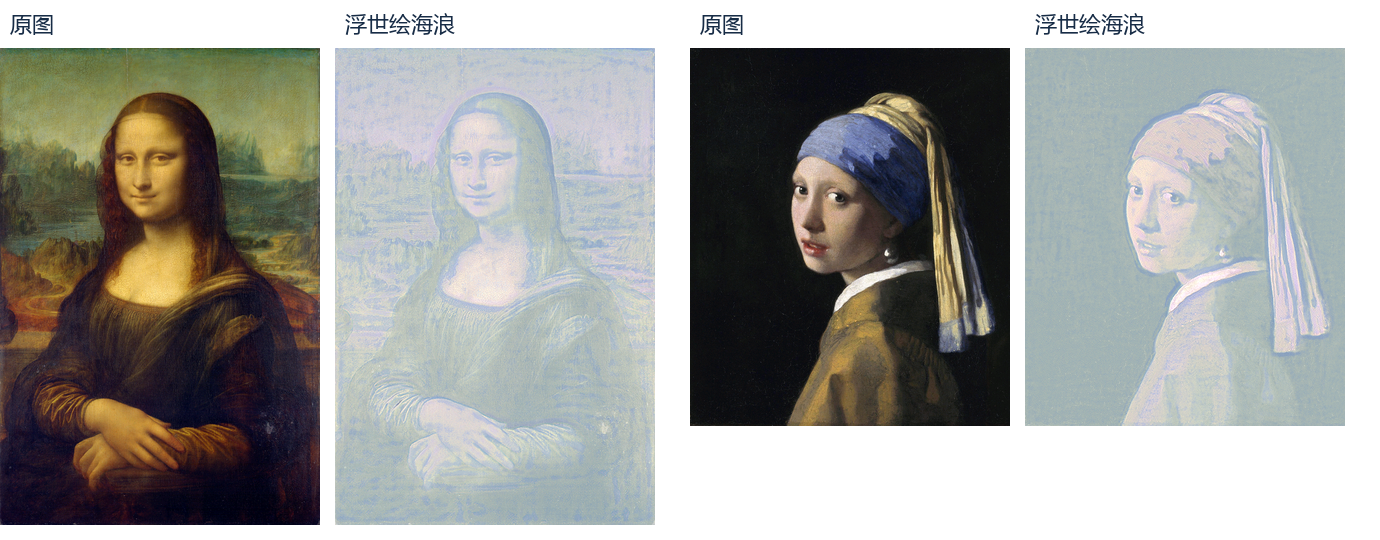
\includegraphics[width=\linewidth]{assets/comparisons/style_01_pairs.png}
\caption{槽1 浮世绘海浪}
\end{figure}

\clearpage
\begin{figure}[H]\centering
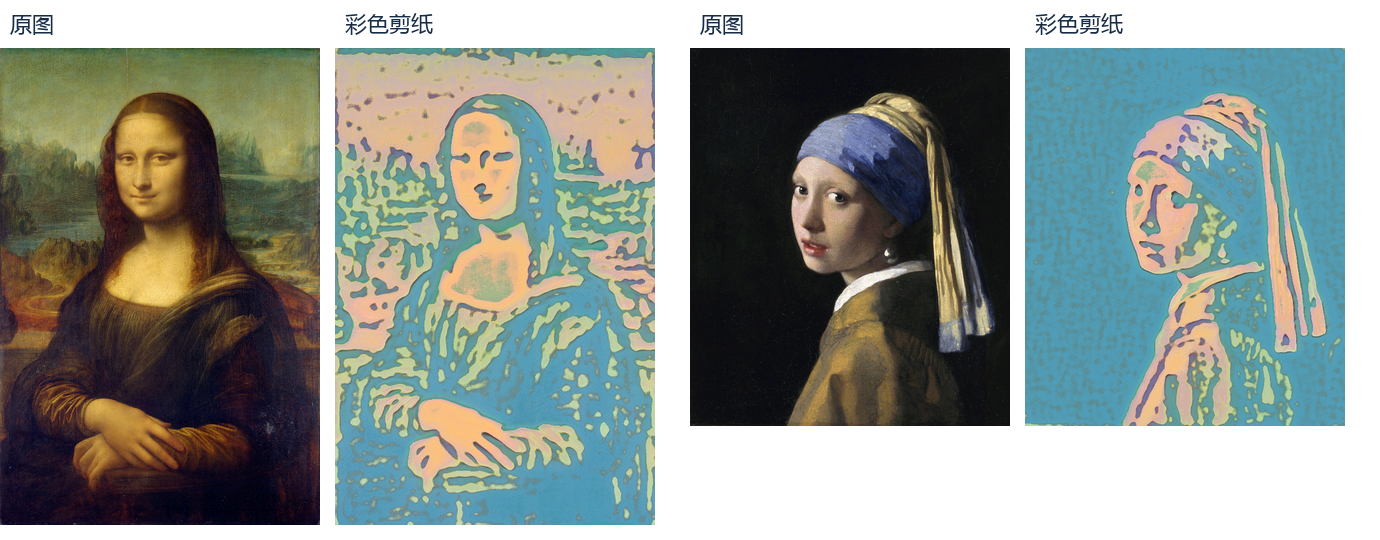
\includegraphics[width=\linewidth]{assets/comparisons/style_02_pairs.png}
\caption{槽2 彩色剪纸}
\end{figure}
\begin{figure}[H]\centering
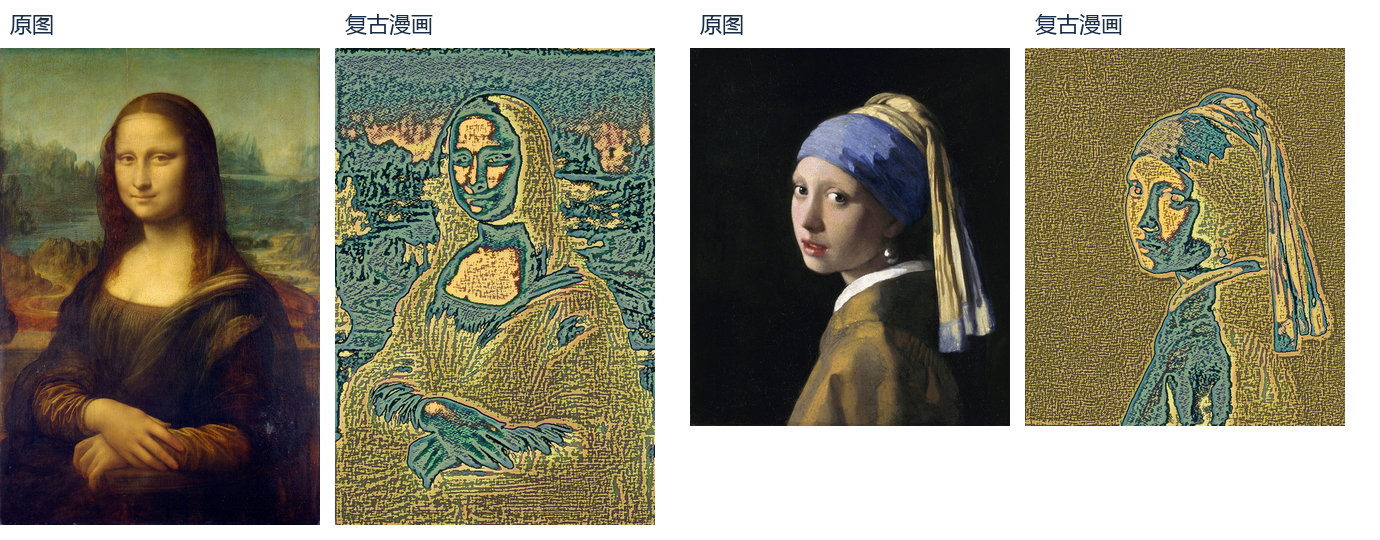
\includegraphics[width=\linewidth]{assets/comparisons/style_03_pairs.png}
\caption{槽3 复古漫画}
\end{figure}

\clearpage
\begin{figure}[H]\centering
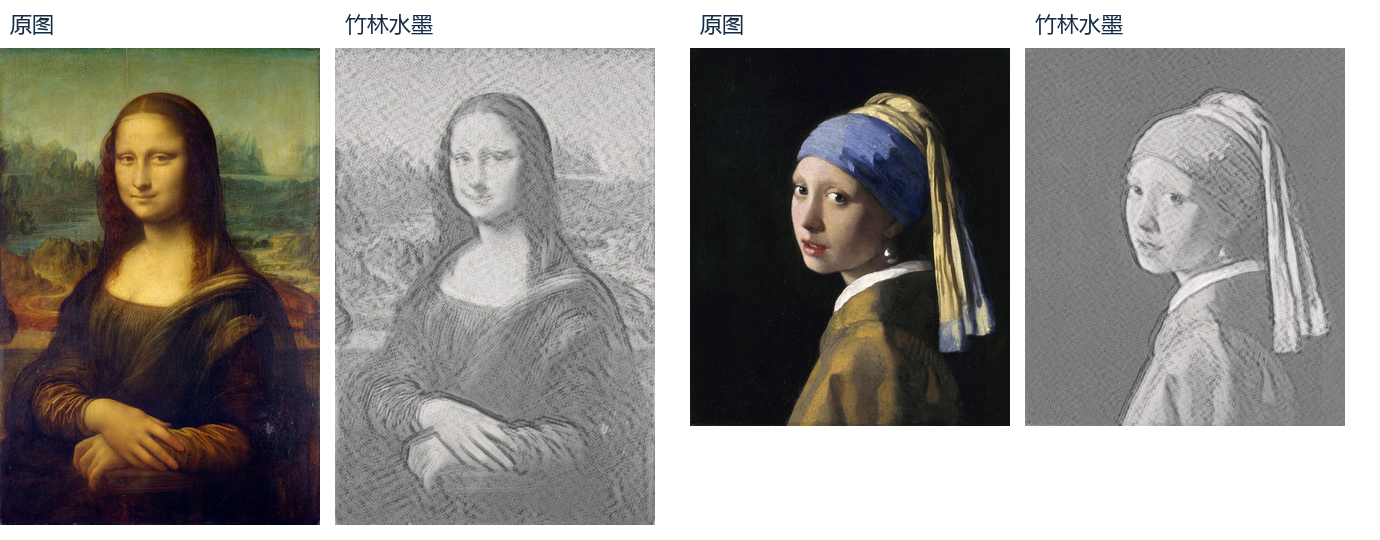
\includegraphics[width=\linewidth]{assets/comparisons/style_04_pairs.png}
\caption{槽4 竹林水墨}
\end{figure}
\begin{figure}[H]\centering
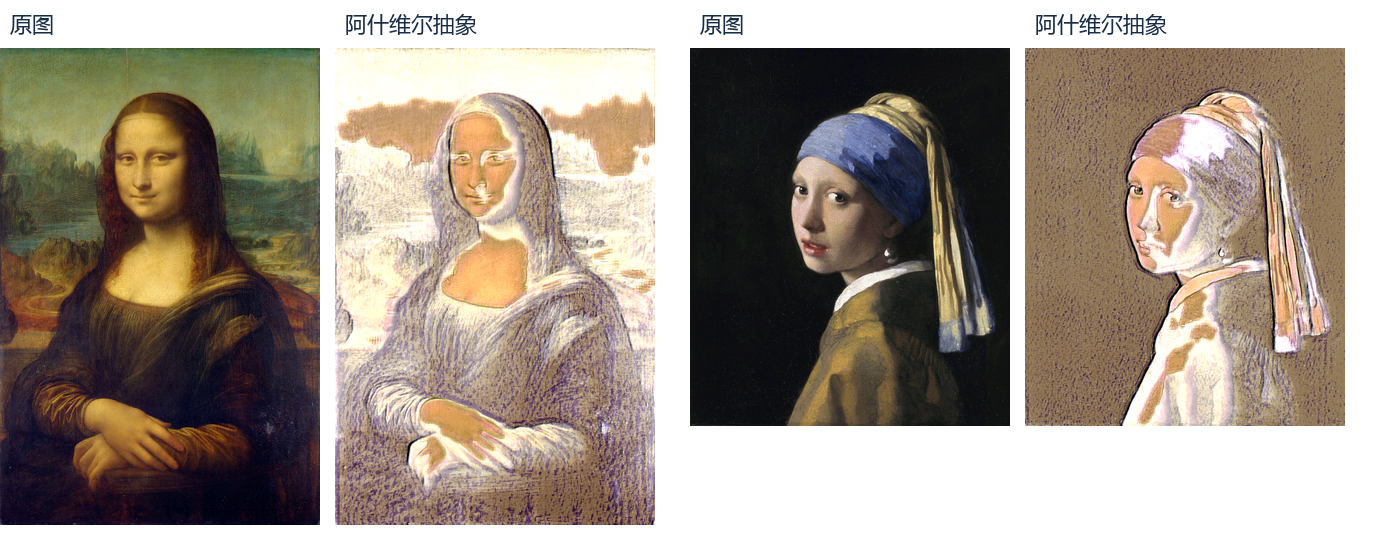
\includegraphics[width=\linewidth]{assets/comparisons/style_05_pairs.png}
\caption{槽5 阿什维尔抽象}
\end{figure}

\clearpage
\begin{figure}[H]\centering
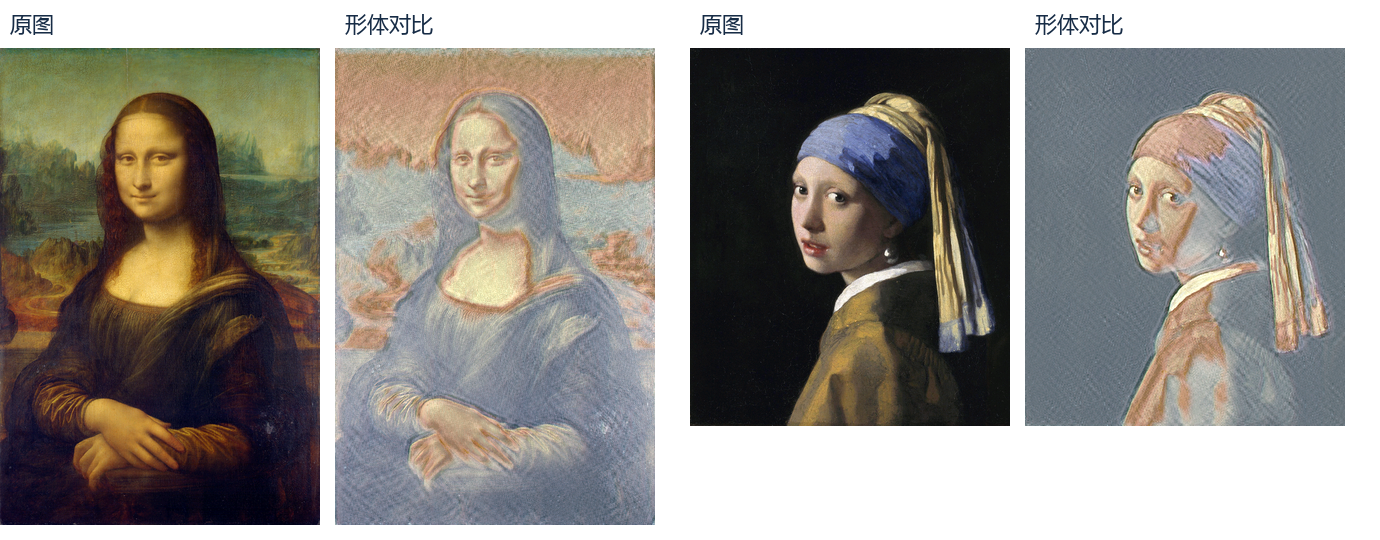
\includegraphics[width=\linewidth]{assets/comparisons/style_06_pairs.png}
\caption{槽6 形体对比}
\end{figure}
\begin{figure}[H]\centering
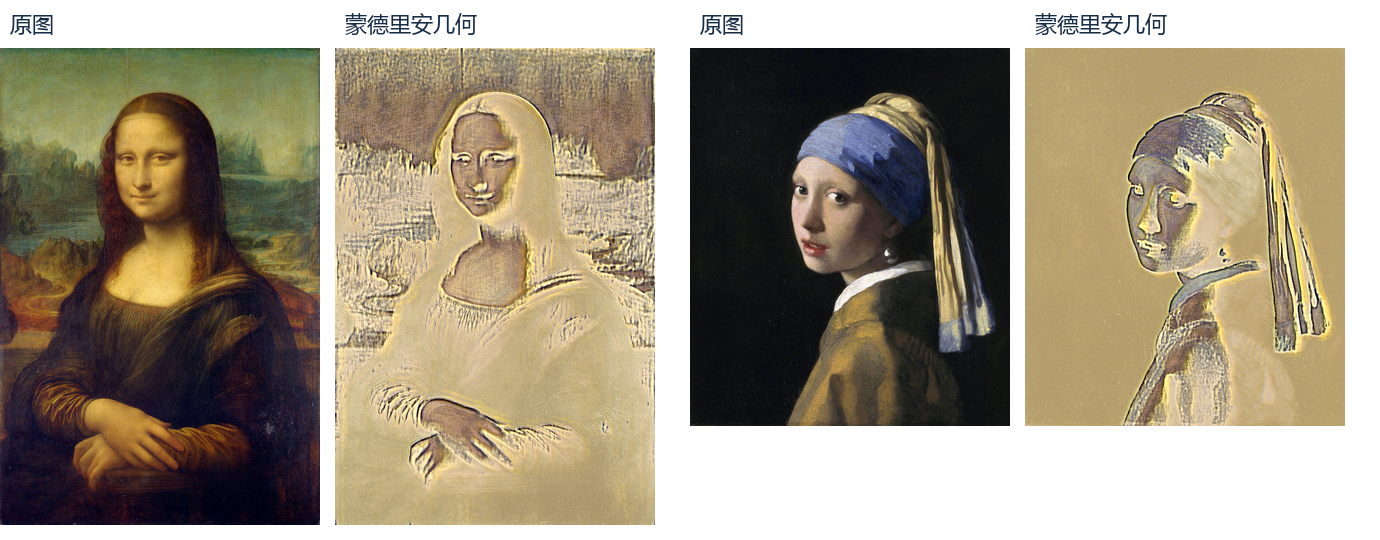
\includegraphics[width=\linewidth]{assets/comparisons/style_07_pairs.png}
\caption{槽7 蒙德里安几何}
\end{figure}

\clearpage
\begin{figure}[H]\centering
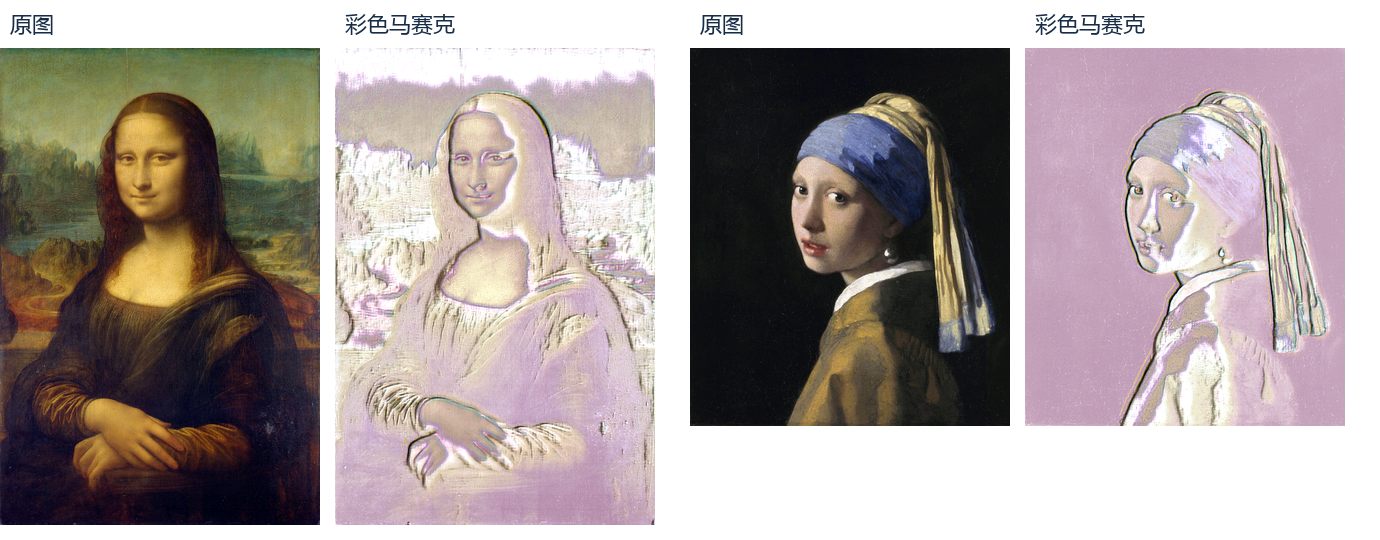
\includegraphics[width=\linewidth]{assets/comparisons/style_08_pairs.png}
\caption{槽8 彩色马赛克}
\end{figure}
\begin{figure}[H]\centering
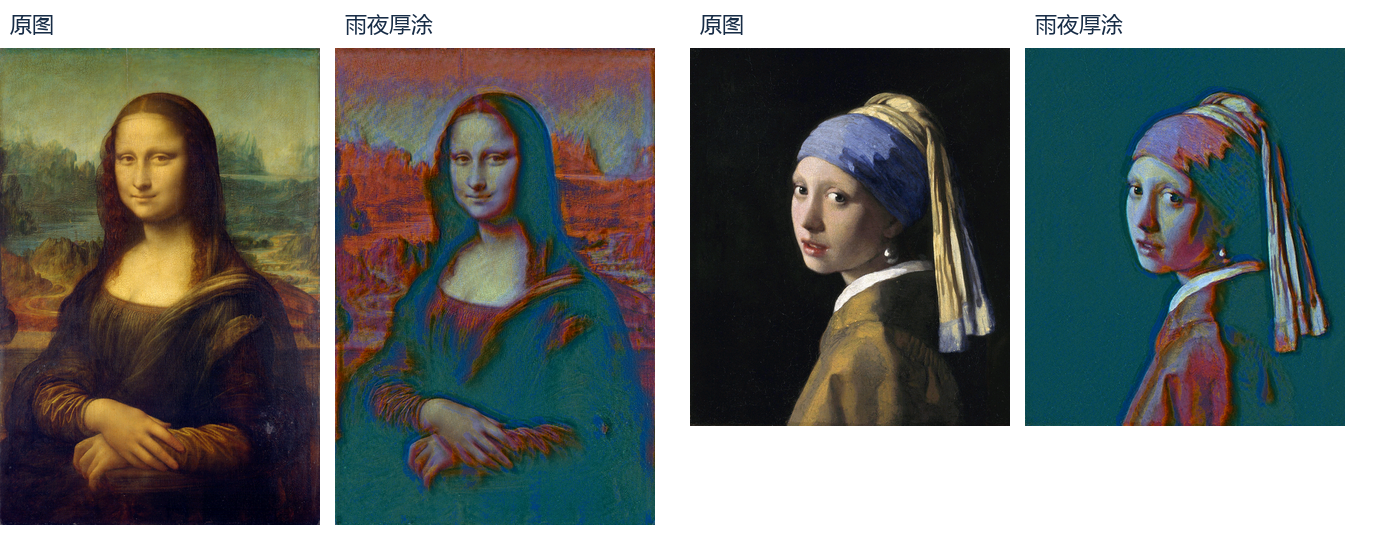
\includegraphics[width=\linewidth]{assets/comparisons/style_09_pairs.png}
\caption{槽9 雨夜厚涂}
\end{figure}

\clearpage
\subsection{实物展示与读数}
\newcommand{\fieldshot}[3]{\begin{minipage}[t]{.48\linewidth}\centering
\IfFileExists{assets/field/#1.jpg}{\includegraphics[width=\linewidth,height=.135\textheight,keepaspectratio]{assets/field/#1.jpg}}{\IfFileExists{assets/field/#1.png}{\includegraphics[width=\linewidth,height=.135\textheight,keepaspectratio]{assets/field/#1.png}}{\fbox{\parbox[c][.122\textheight][c]{.91\linewidth}{\centering\textcolor{teal}{\textbf{#1}}\par\small 待补实拍}}}}
\par\smallskip{\small\bfseries #2}\par{\footnotesize #3}\end{minipage}}
\noindent\fieldshot{P01}{原图与装置}{同框保留SC431HAI、开发板、HDMI屏及原场景。}\hfill
\fieldshot{P02}{风格图}{固定机位，记录风格S和一处可辨识的纹理。}
\par\medskip\noindent\fieldshot{P03}{同源左右对比}{让物体横跨中线，观察两侧轮廓与运动是否衔接。}\hfill
\fieldshot{P04}{手势确认}{完整的手置于框中，记录候选G及进度P；视频保留确认过程。}
\par\medskip\noindent\fieldshot{P05}{UI开启}{记录屏上完整字段及手势确认后的前台槽S。}\hfill
\fieldshot{P06}{UI关闭}{同一视图按KEY3，以相同机位记录干净画面。}
\par\medskip
\noindent C为一秒内发布的好采集帧数，I为完成的新风格推理帧数，H60表示配置的HDMI刷新率。G为投票后的候选数字，短横线表示暂无候选。P为已经持续的完整秒数，范围0--4。S为已经提交到前台的风格槽号。录入时，L显示当前标签，A显示已经接受的样本数量。青框标出镜头中采样手势的区域。
\clearpage
\blocktitle{名画输入的实屏对照}
\noindent\fieldshot{P07}{《蒙娜丽莎》}{十风格摄像头版，镜头采集原画，KEY3关闭UI。}\hfill
\fieldshot{P08}{《戴珍珠耳环的少女》}{十风格摄像头版，固定机位，记录实际风格槽。}
\par\bigskip
\noindent\fieldshot{U01}{串口输入《蒙娜丽莎》}{UART四风格验证工程，上传源图后在板上转换。}\hfill
\fieldshot{U02}{串口输入《戴珍珠耳环的少女》}{UART四风格验证工程，记录板上按键选择。}
\par\bigskip
摄像头图组包含光照、镜头曝光、白平衡与显示器再拍摄的影响。串口图组采用确定的RGB565输入和四风格模型。两条路径分别标记，便于说明色差和纹理差异来自哪一环节。

\blocktitle{板端运行记录}
采集与推理按完整帧计数。切换延迟取按键消抖完成至新风格前台生效的时间差。
\begin{center}\small\begin{tabularx}{\linewidth}{@{}p{.36\linewidth}XX@{}}\toprule
测量项 & 槽0风格图 & 槽4左右对比\\\midrule
时间窗 / 好采集帧增量 & 待测 & 待测\\
推理FPS均值 / 最低一秒 & 待测 & 待测\\
跳过源帧 / 坏帧 / 显示欠载 & 待测 & 待测\\
风格切换延迟 / 样本数 & 待测 & 待测\\\bottomrule
\end{tabularx}\end{center}
